\documentclass[serif]{beamer}
\usetheme{CambridgeUS}
\usepackage{ctex}
\usepackage{amsmath,amssymb,amsfonts,bm}
\usepackage{graphicx,subfigure}
\usepackage{adjustbox}
\usepackage{color,xcolor}

% 自定义数学公式
\newcommand{\abs}[1]{\left\vert#1\right\vert}
\newcommand{\floor}[1]{\left\lfloor{#1}\right\rfloor}
\newcommand{\ceil}[1]{\left\lceil{#1}\right\rceil}
\newcommand{\sbrace}[1]{\left(#1\right)}
\newcommand{\mbrace}[1]{\left[#1\right]}
\newcommand{\bbrace}[1]{\left\{#1\right\}}
\newcommand{\eval}[2]{\left.{#1}\right|_{#2}}
\newcommand{\conj}[1]{{\rm conj}\sbrace{#1}}
\newcommand{\ALLP}{\mathcal{A}}
\newcommand{\PS}{\mathcal{P}}
\newcommand{\dd}[1]{\mathrm{d}#1}
\newcommand{\ii}[1]{\int\!{#1\dd x}}
\newcommand{\VecNorm}[1]{\left\Vert#1\right\Vert}% 向量模
\newcommand{\spell}[1]{#1}
\newcommand{\up}[1]{^{(#1)}}
\newcommand{\TT}{^\top}% 矩阵转置
\newcommand{\OO}{\ensuremath{\mathbb O}}% n 阶展开多项式余项
\newcommand{\OC}{\ensuremath{\mathcal O}}% 算法复杂度
\newcommand{\lfrac}[2]{#1/#2}
\newcommand{\DIF}[1]{\ensuremath{\frac{\partial}{\partial #1}}}
\newcommand{\DIFF}[2]{\ensuremath{\frac{\partial #1}{\partial #2}}}

\newcommand{\Painleve}{Painlev{\'e}}

\title[华东师范大学硕士学位论文]{非线性系统的精确解及其\\ 基础算法的符号计算研究}
\author[余江涛]{余江涛 \and \\导师: 柳银萍~教授}
\date{\today}

\begin{document}
\frame{\titlepage}

\section{本文工作}
\begin{frame}
\frametitle{本文工作}
\begin{figure}
\centering
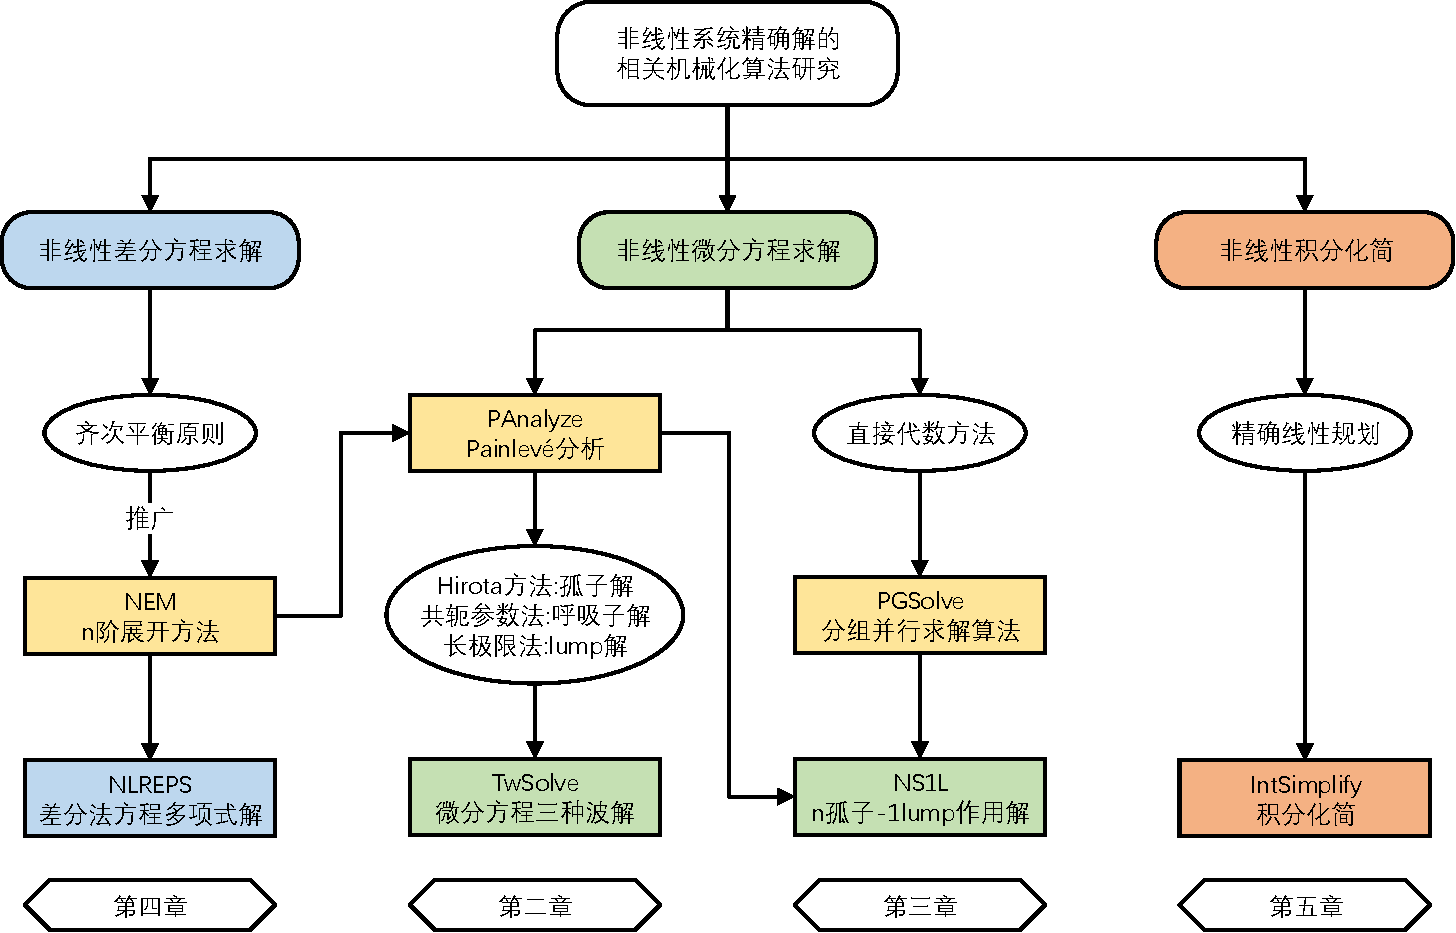
\includegraphics[width=\textwidth]{../paper/fig/outline.pdf} 
\end{figure}
\end{frame}

\section{非线性演化方程的三种波解}
\begin{frame}
\frametitle{非线性演化方程的三种波解}
\begin{enumerate}
\item \Painleve{}展开法得到变换.
\item 简单 Hirota 方法得到孤子解.
\item 共轭参数法得到呼吸子解.
\item 长极限法得到 lump 解.
\end{enumerate}
\end{frame}

\subsection{\Painleve{}展开法}
\begin{frame}
\frametitle{\Painleve{}展开法}
\end{frame}

\subsection{Hirota 方法与孤子解}
\begin{frame}
\frametitle{Hirota 方法与孤子解}
\end{frame}

\subsection{共轭参数法与呼吸子解}
\begin{frame}
\frametitle{共轭参数法与呼吸子解}
\end{frame}

\subsection{长极限法与 lump 解}
\begin{frame}
\frametitle{长极限法与 lump 解}
\end{frame}

\subsection{应用实例}
\begin{frame}
\frametitle{应用实例}
(3+1)JM方程
\begin{equation*}
    u_{xxxy}+3u_{xx}u_y+3u{x}u_{xy}+2u_{ty}-3u_{xz}=0. 
\end{equation*}
\begin{figure}
\centering 
\subfigure[1-孤子解 \label{jm:1-soliton}]{
    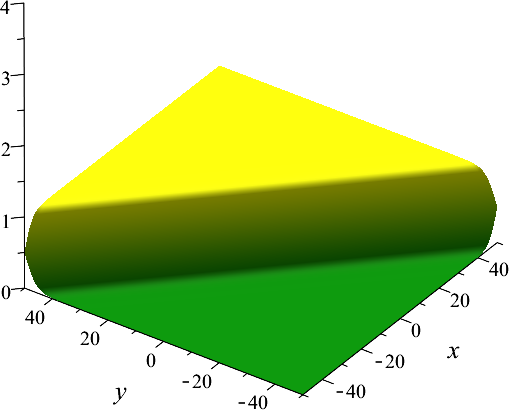
\includegraphics[width=.3\textwidth]{../paper/fig/(3+1)JM-1-soliton.png}    
}
\subfigure[2-孤子解 \label{jm:2-soliton}]{
    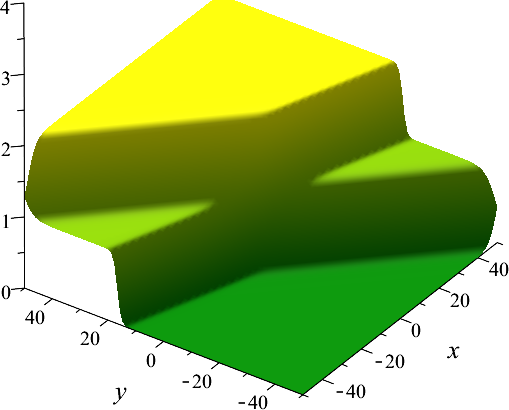
\includegraphics[width=.3\textwidth]{../paper/fig/(3+1)JM-2-soliton.png}
}
\subfigure[3-孤子解 \label{jm:3-soliton}]{
    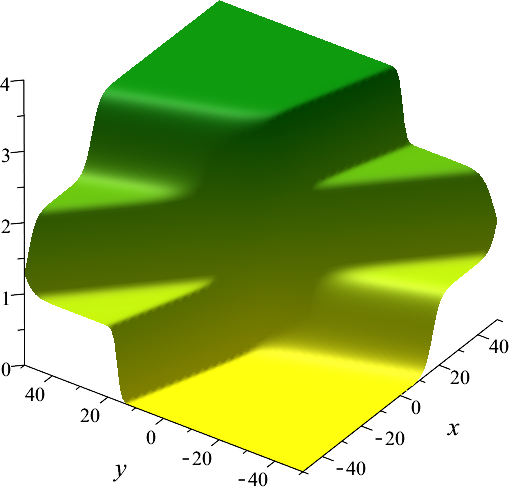
\includegraphics[width=.3\textwidth]{../paper/fig/(3+1)JM-3-soliton.png}
}
\end{figure}
\end{frame}

\begin{frame}
\begin{figure}
\centering 
\subfigure[1-呼吸子解 \label{jm:1-breather}]{
    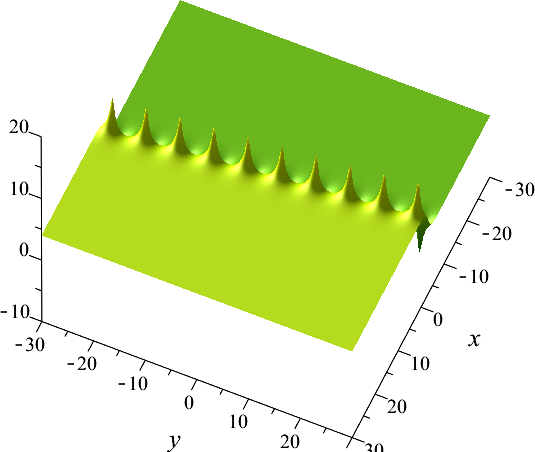
\includegraphics[width=.3\textwidth]{../paper/fig/(3+1)JM-1-breather.png}
}
\subfigure[2-呼吸子解 \label{jm:2-breather}]{
    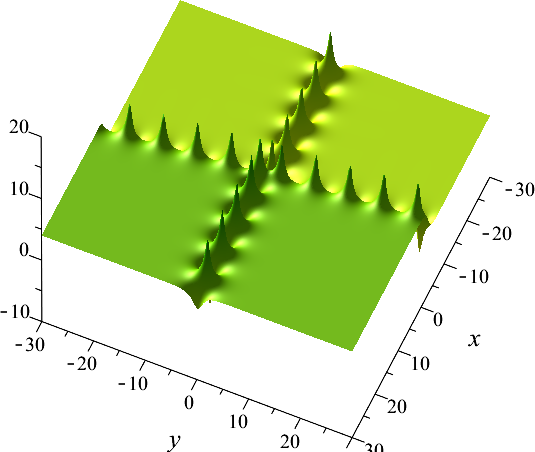
\includegraphics[width=.3\textwidth]{../paper/fig/(3+1)JM-2-breather.png}
}
\subfigure[3-呼吸子解 \label{jm:3-breather}]{
    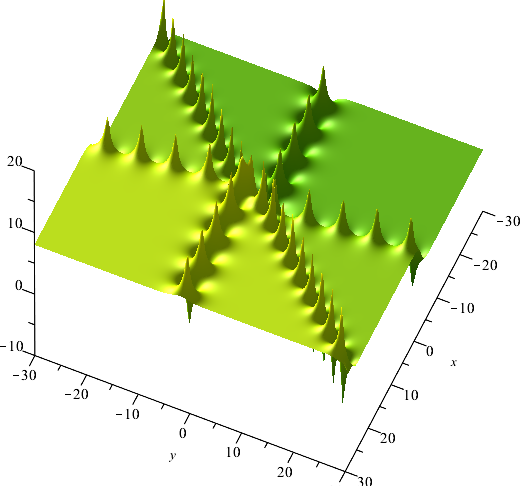
\includegraphics[width=.3\textwidth]{../paper/fig/(3+1)JM-3-breather.png}
}
\subfigure[1-lump解 \label{jm:1-lump}]{
    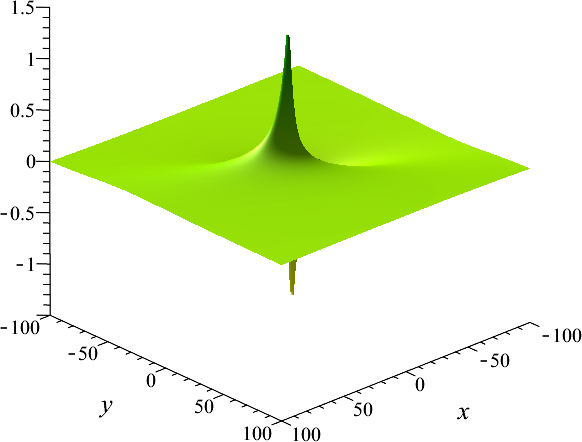
\includegraphics[width=.3\textwidth]{../paper/fig/(3+1)JM-1-lump.png}
}
\subfigure[2-lump解 \label{jm:2-lump}]{
    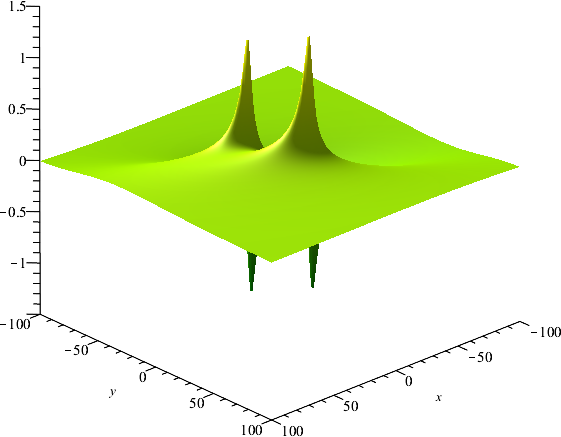
\includegraphics[width=.3\textwidth]{../paper/fig/(3+1)JM-2-lump.png}
}
\subfigure[3-lump解 \label{jm:3-lump}]{
    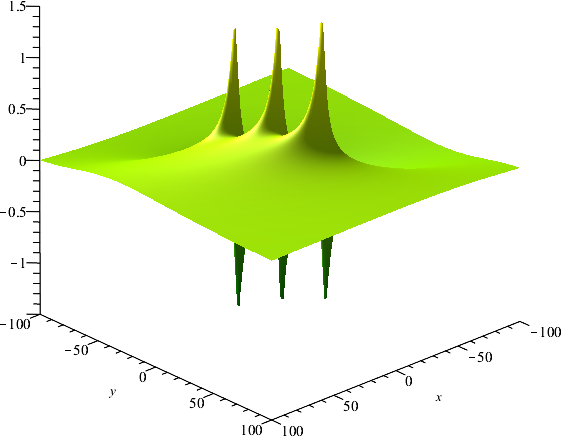
\includegraphics[width=.3\textwidth]{../paper/fig/(3+1)JM-3-lump.png}
}
\end{figure}
\end{frame}

\subsection{实验与分析}
\begin{frame}
\frametitle{实验与分析}
\end{frame}

\section{分组并行求解算法及其应用}
\begin{frame}
\frametitle{分组并行求解算法及其应用}
\begin{enumerate}
\item PGSolve: 分组并行算法
\item NS1L: 求n孤子-1 lump相互作用解的软件包
\end{enumerate}
\end{frame}

\subsection{PGSolve: 分组并行求解算法}
\begin{frame}
\frametitle{PGSolve: 分组并行求解算法}
\begin{figure}
\centering
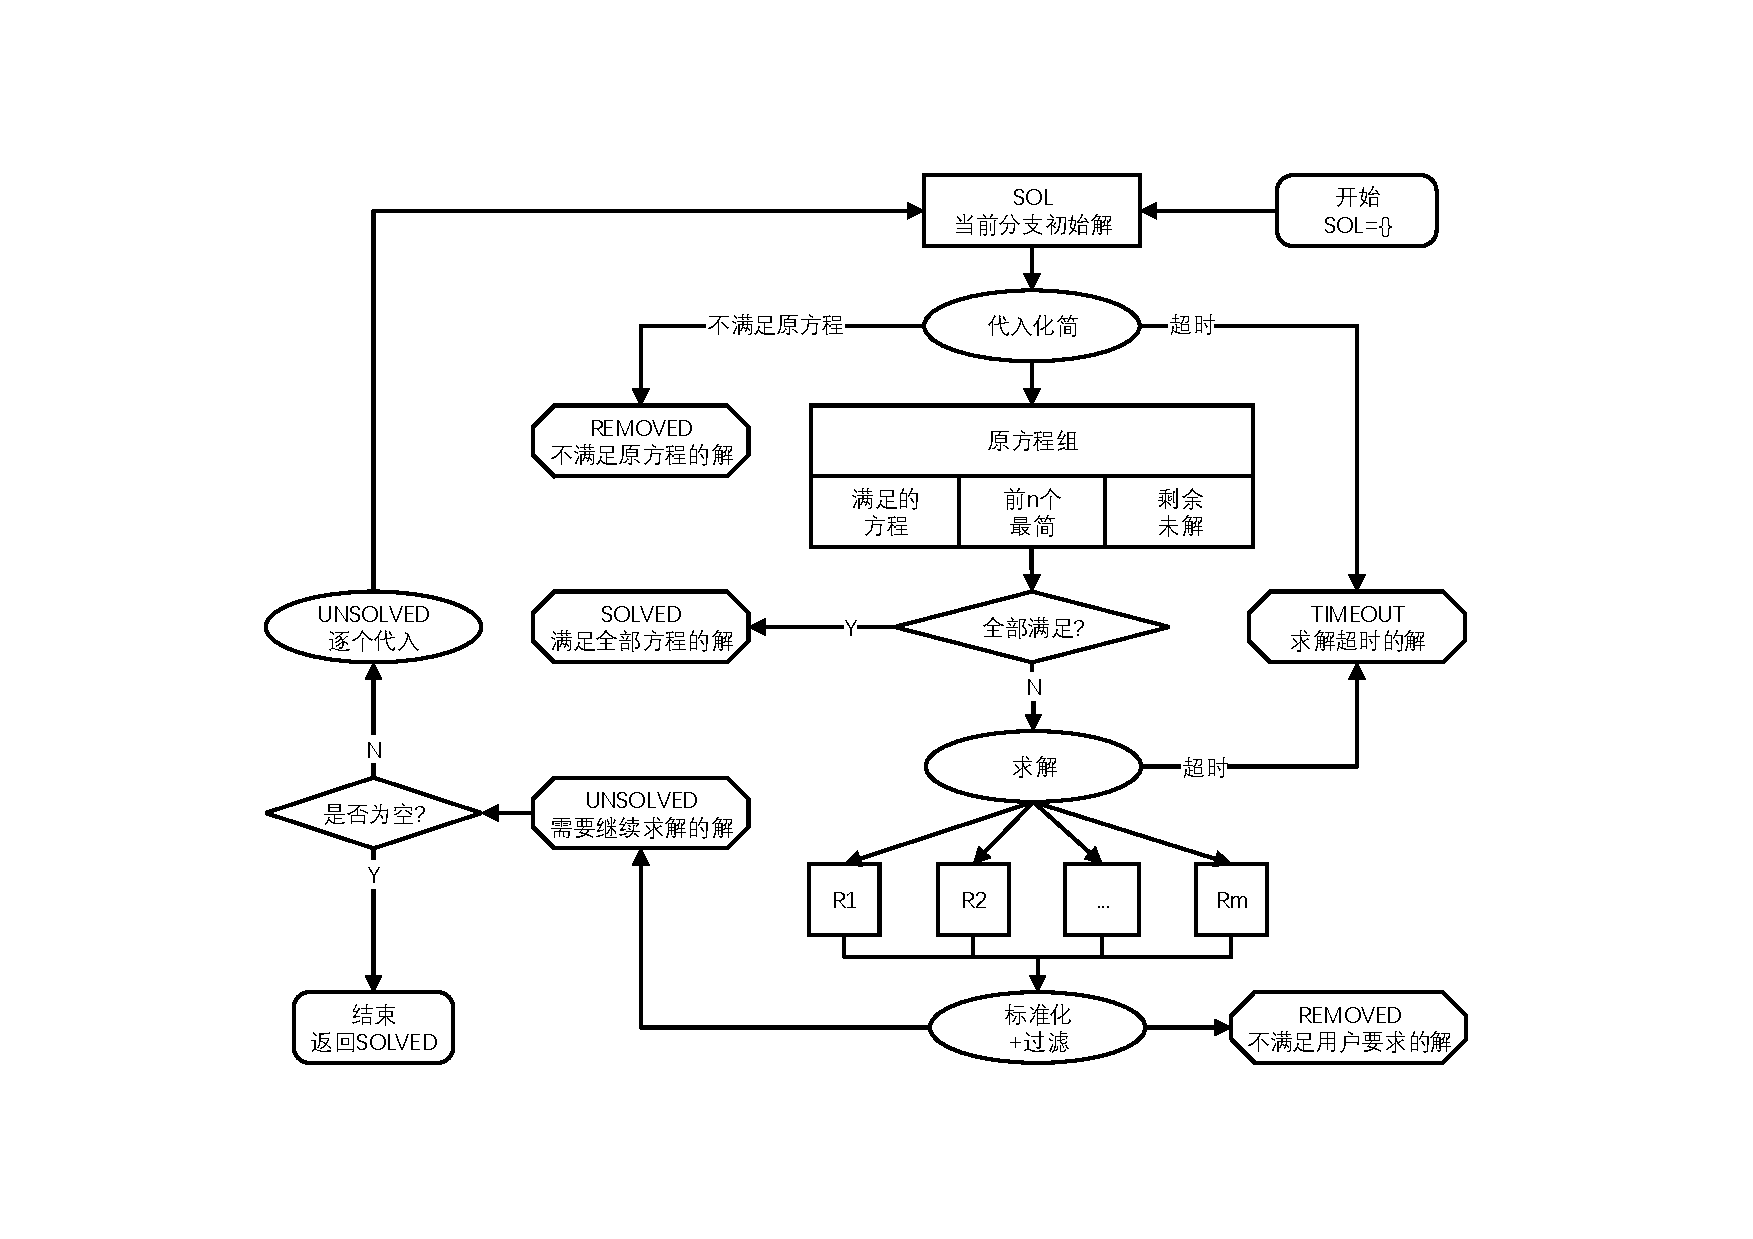
\includegraphics[height=0.8\textheight]{../paper/fig/pgsolve.pdf}
\end{figure}
\end{frame}

\subsection{NS1L: 求n孤子-1 lump相互作用解的软件包}
\begin{frame}
\frametitle{NS1L: 求n孤子-1 lump相互作用解的软件包}
\end{frame}

\begin{frame}
\begin{adjustbox}{max width=\textwidth}
\renewcommand{\arraystretch}{1.3}
\begin{tabular}{cccccc}
\hline
方程名称    & 解的阶数 & 方程数量 & 分组大小 & 解的个数 & 运行时间(s) \\ 
\hline 
(2+1)SK & 0 & 20 & 5 & 1 & 1.875 \\
(2+1)SK & 1 & 65 & 3 & 1 & 3.154 \\
(2+1)SK & 2 & 179 & 5 & 2 & 12.926 \\
(2+1)BKP-T & 0 & 20 & 5 & 1 & 1.036 \\
(2+1)BKP-T & 1 & 65 & 3 & 1 & 3.181 \\
(2+1)BKP-T & 2 & 179 & 5 & 2 & 12.749 \\
(3+1)YTSF & 0 & 35 & 5 & 3 & 2.891 \\
(3+1)YTSF & 1 & 120 & 5 & 3 & 8.713 \\
(3+1)YTSF & 2 & 324 & 5 & 3 & 38.527 \\
(3+1)JM & 0 & 35 & 5 & 4 & 3.120 \\
(3+1)JM & 1 & 120 & 5 & 6 & 14.910 \\
(3+1)JM & 2 & 324 & 5 & 5 & 81.711 \\
\hline 
\end{tabular}
\end{adjustbox}
\end{frame}

\section{非线性差分方程精确解与$n$阶展开方法}
\begin{frame}
\frametitle{非线性差分方程精确解与$n$阶展开方法}
\end{frame}

\begin{frame}
\begin{figure}
\centering
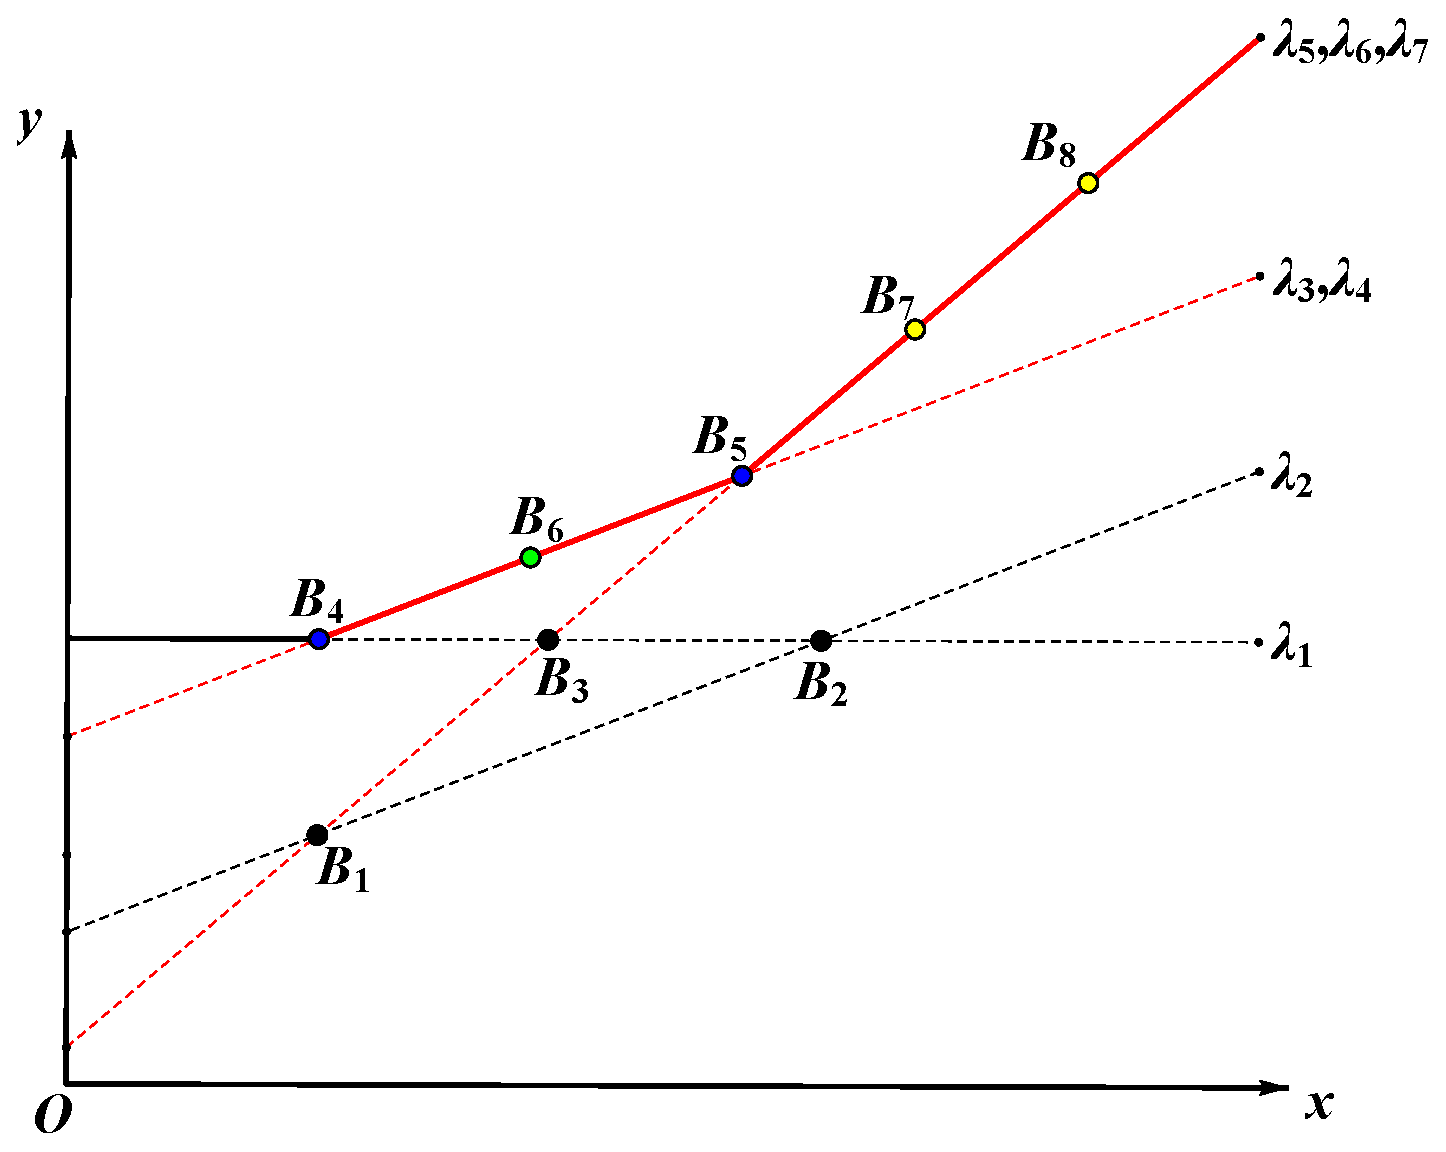
\includegraphics[height=0.9\textheight]{../paper/fig/ps.eps}
\end{figure}
\end{frame}

\section{$n$阶展开方法在微分方程求解中的应用}
\begin{frame}
\frametitle{$n$阶展开方法在微分方程求解中的应用}
\begin{enumerate}
\item NCTM: 在双曲正切方法中的应用
\item PAnalyze: 在\Painleve{}展开法中的应用
\end{enumerate}
\end{frame}

\begin{frame}
\begin{equation*}
\begin{split}
& \DIF{t}F\sbrace{x,m,u\up{n}}  \\
=& \DIF{t}\sbrace{\sum_{k=0}^{n-1}{u_k x^{m-k}}+\OO(x^{m-n})} \\
=& \sum_{k=0}^{n-1}{\DIFF{u_k}{t}x^{m-k}}+\DIFF{x}{t}\cdot\sum_{k=0}^{n-1}{u_k (m-k) x^{m-k-1}}+\DIFF{x}{t}\cdot\OO(x^{m-n-1}) \\
=& \sum_{k=0}^{n-1}{\DIFF{u_k}{t}x^{m-k}}+\DIFF{x}{t}\cdot\sbrace{\sum_{k=0}^{n-1}{u_k (m-k) x^{(m-1)-k}}+\OO\sbrace{x^{(m-1)-n)}}} \\ 
=& F\sbrace{x,m,v\up{n}}+{\color{red}\DIFF{x}{t}}\cdot F\sbrace{x,m-1,w\up{n}}.
\end{split}
\end{equation*}
\end{frame}

\subsection{NCTM: 在双曲正切方法中的应用}
\begin{frame}
\frametitle{NCTM: 在双曲正切方法中的应用}
\end{frame}

\subsection{PAnalyze: 在\Painleve{}展开法中的应用}
\begin{frame}
\frametitle{PAnalyze: 在\Painleve{}展开法中的应用}
\end{frame}

\section{非线性积分表达式化简}
\begin{frame}
\frametitle{非线性积分表达式化简}
\end{frame}

\section{总结}
\begin{frame}
\frametitle{总结}
\begin{figure}
\centering
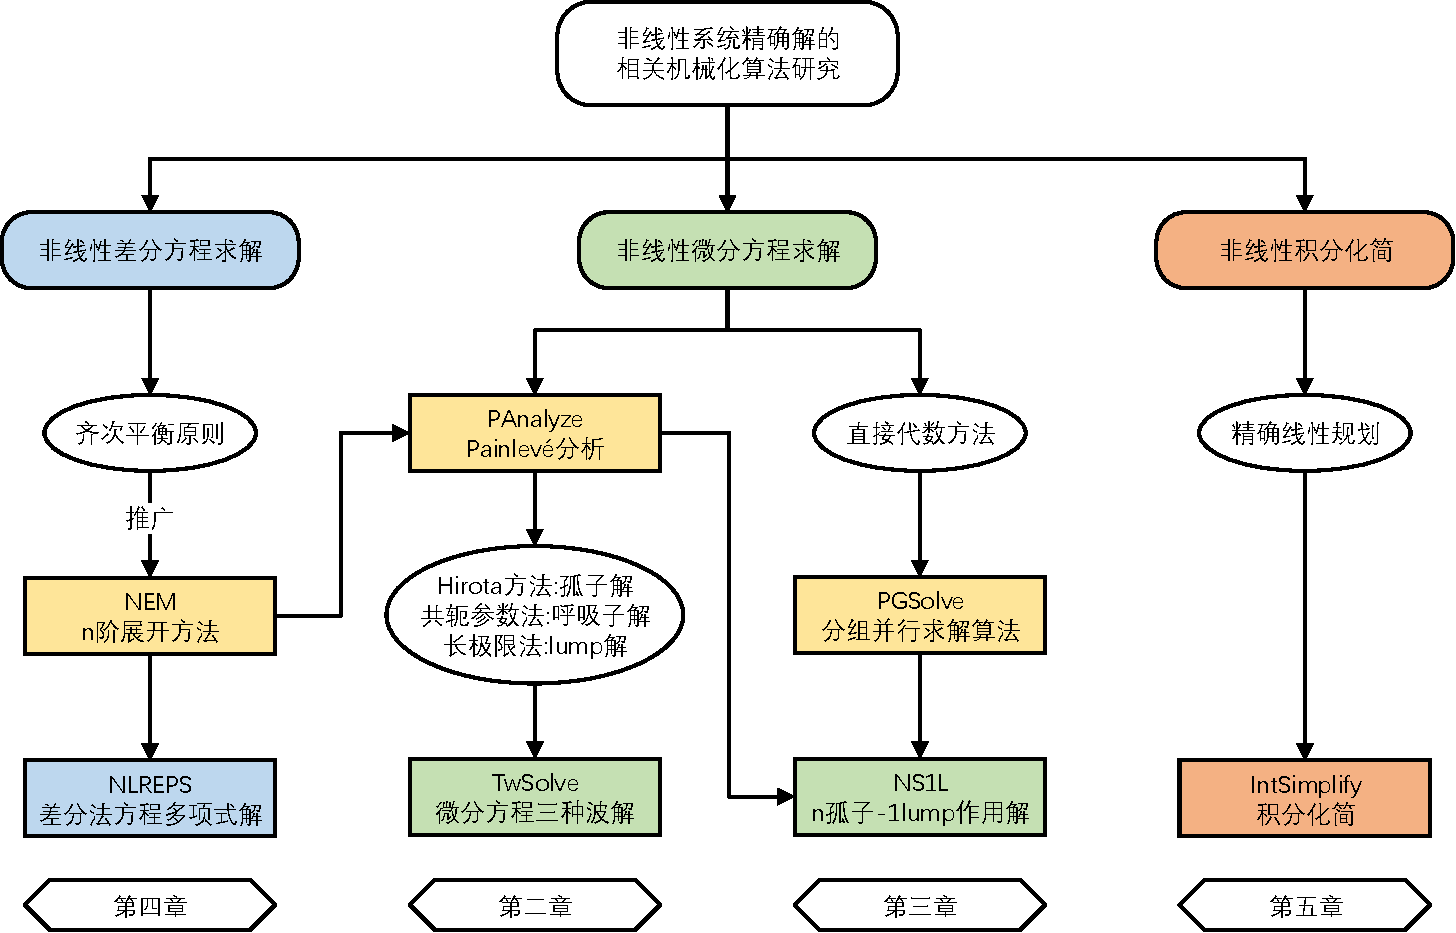
\includegraphics[width=\textwidth]{../paper/fig/outline.pdf} 
\end{figure}
\end{frame}

\section{致谢}
\begin{frame}
\centerline{\Huge 谢谢}
\end{frame}
\end{document}